\documentclass[10pt]{article}
\usepackage[letterpaper,margin=0.58in]{geometry}
\usepackage[T1]{fontenc}
\usepackage{lmodern}
\usepackage{microtype}
\usepackage{graphicx}
\usepackage{booktabs}
\usepackage{tabularx}
\usepackage{array}
\usepackage{enumitem}
\usepackage{xcolor}
\usepackage[hidelinks]{hyperref}
\usepackage{fancyhdr}

\definecolor{navy}{HTML}{153B50}
\definecolor{teal}{HTML}{159A9C}
\definecolor{amber}{HTML}{D98E04}
\definecolor{soft}{HTML}{EEF5F5}
\definecolor{ink}{HTML}{17242B}
\newcommand{\pq}{\mathrm{PQ}}
\newcommand{\scopebox}[1]{%
  \noindent\colorbox{soft}{\parbox{0.965\linewidth}{\small #1}}}
\setlist[itemize]{leftmargin=1.3em,itemsep=1.5pt,topsep=2pt}
\setlength{\parindent}{0pt}
\setlength{\parskip}{3.5pt}
\pagestyle{fancy}
\fancyhf{}
\lhead{\small\textcolor{navy}{TessScope}}
\rhead{\small\textcolor{navy}{Tesseract Hackathon 2026 -- Track 05}}
\cfoot{\small\thepage\ / 4}
\renewcommand{\headrulewidth}{0.3pt}

\begin{document}

\begin{center}
  {\fontsize{23}{25}\selectfont\bfseries\textcolor{navy}{TessScope}}\\[2pt]
  {\large Exact cross-runtime gradients for closed-loop microscope co-design}\\[4pt]
  {\small Tesseract Hackathon 2026 -- Track 05 -- Differentiable graphics \& rendering}
\end{center}

\textbf{The problem.} A fluorescence microscope pupil that preserves nucleus
segmentation tends to erase depth cues, while a pupil that makes signed defocus obvious
can distort nuclei. TessScope co-designs one bounded phase-only pupil for the complete
two-exposure decision loop rather than optimizing image sharpness in isolation.

\textbf{Protected validation claim.} TessScope uses exact gradients across
JAX/Chromatix optics, NumPy/SciPy autofocus, and PyTorch/InstanSeg to causally improve
closed-loop correction over a forward-identical stopped-gradient system.

\begin{center}
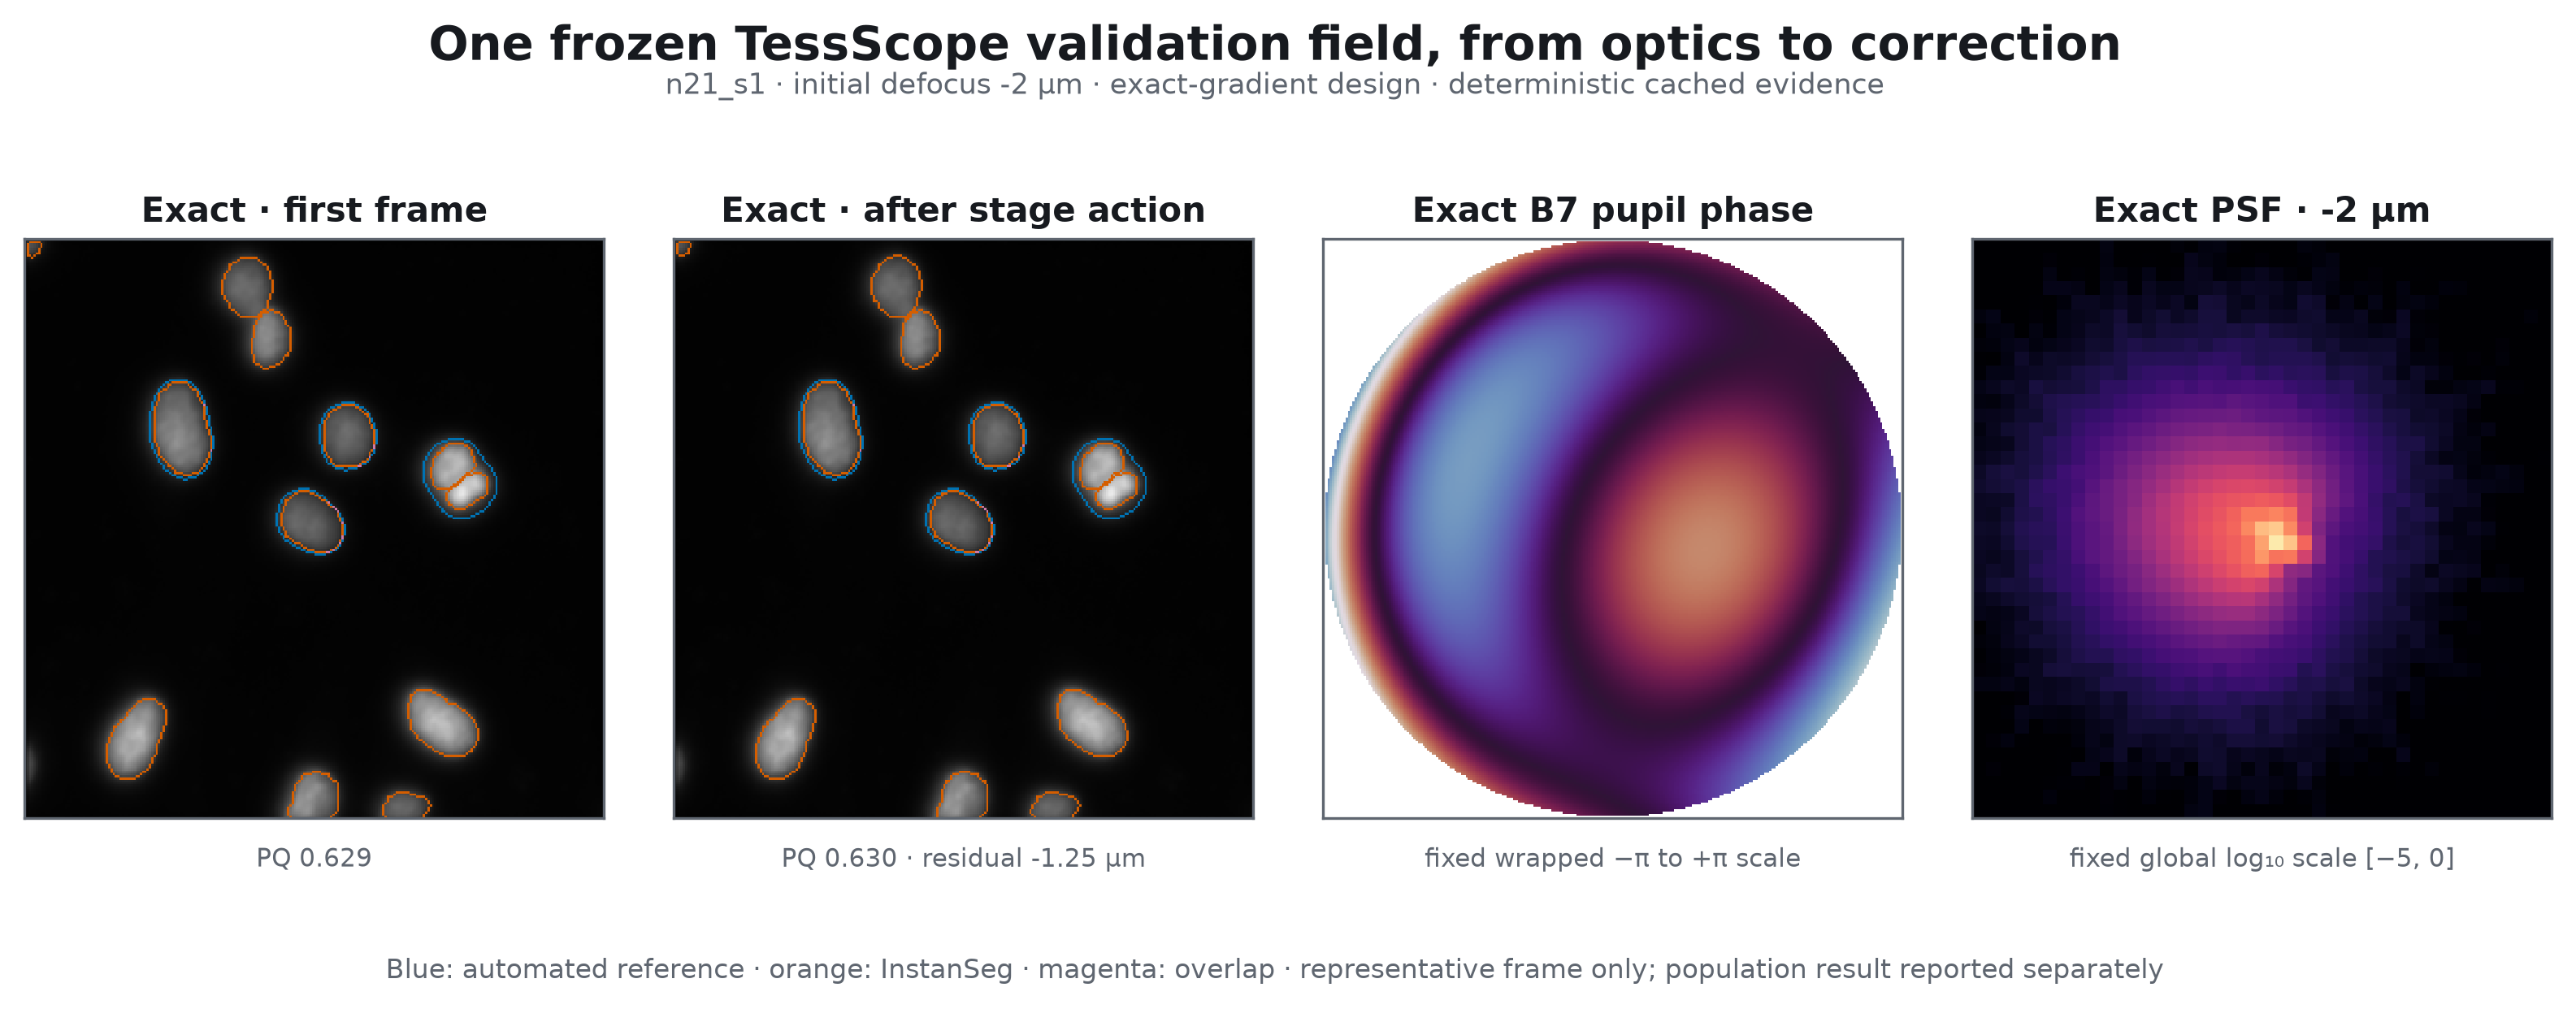
\includegraphics[width=0.96\linewidth]{../../outputs/demo/figures/hero-evidence.png}
\end{center}

\vspace{-4pt}
\begin{tabularx}{\linewidth}{>{\bfseries}p{0.28\linewidth} >{\raggedleft\arraybackslash}p{0.18\linewidth} X}
\toprule
Measure & Result & Meaning \\
\midrule
First hard off-focus PQ & 0.492192 & Before the predicted stage move \\
Corrected hard off-focus PQ & \textbf{0.552295} & One bounded predicted correction later \\
Focus error & 1.267923 $\mu$m & 98.89\% signed-direction accuracy \\
Exact vs. stopped & \textbf{+0.006259 PQ} & 95\% well-bootstrap CI [+0.000670, +0.011547] \\
Exact vs. piecewise-028 & +0.001285 PQ & CI [-0.001719, +0.004800]; not significant \\
\bottomrule
\end{tabularx}

\scopebox{\textbf{Scope.} PQ is panoptic quality on a 0--1 scale, not percent accuracy.
All displayed v2 evidence is validation-only. The locked BBBC006 test remains sealed.
No physical microscope or fabricated phase mask has validated the system.}

\newpage
\section*{One differentiable program, three native runtimes}

\begin{center}
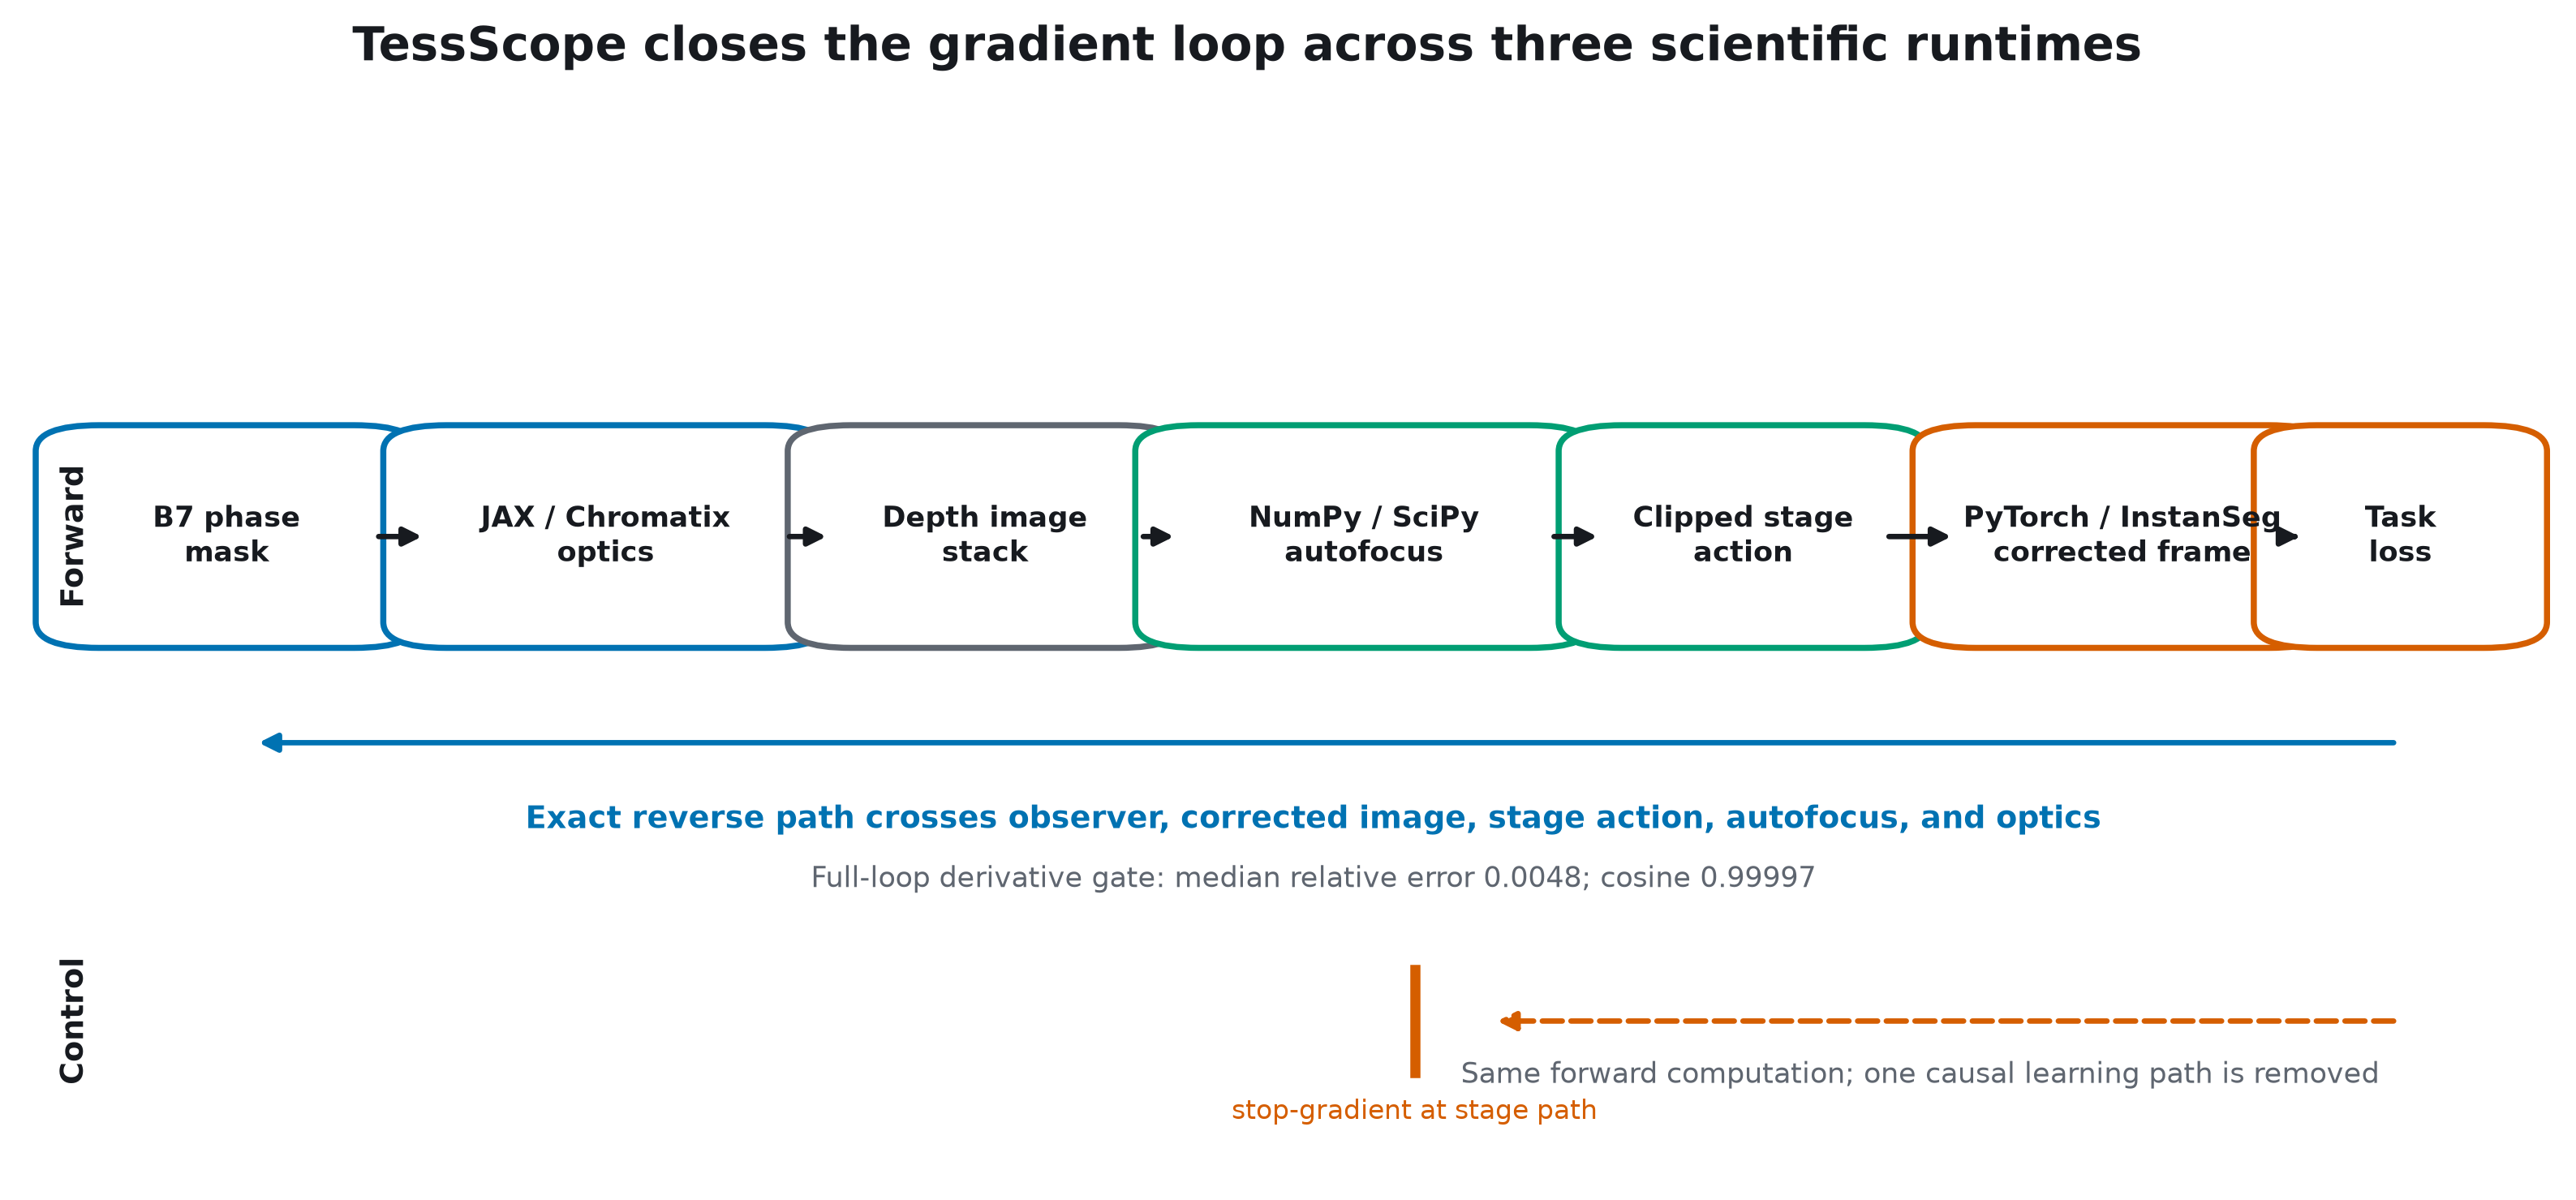
\includegraphics[width=0.96\linewidth]{../../outputs/demo/figures/gradient-architecture.png}
\end{center}

\vspace{-5pt}
\begin{tabularx}{\linewidth}{>{\bfseries}p{0.19\linewidth} p{0.20\linewidth} X p{0.23\linewidth}}
\toprule
Tesseract & Native stack & Forward role & Reverse path \\
\midrule
Optics & JAX + Chromatix & Phase pupil and depth-dependent fluorescence formation; called for both exposures & JAX VJP through pupil and residual depth \\
Autofocus & NumPy + SciPy & Spectral features, signed-z ridge fit, clipped stage action & Analytic feature VJP and implicit ridge-solve VJP \\
Observer & PyTorch + InstanSeg & Frozen nucleus task loss on first and corrected frames & PyTorch autograd input VJP \\
\bottomrule
\end{tabularx}

\textbf{Why Tesseract is load-bearing.} Each component stays in its tested scientific
ecosystem. Tesseract supplies typed service boundaries and derivative endpoints;
\texttt{tesseract-jax} exposes remote calls as a JAX-differentiable program. One objective
therefore returns one pupil gradient through JAX $\rightarrow$ SciPy $\rightarrow$ JAX
$\rightarrow$ PyTorch without reimplementing the models in a single framework.

\textbf{Closed-loop computation.}
\begin{enumerate}[leftmargin=1.45em,itemsep=1.5pt,topsep=2pt]
  \item The bounded seven-parameter pupil forms an initial seven-plane stack.
  \item Two support fields fit a signed-depth autofocus model; the query predicts a
        stage move clipped to $[-6,+6]~\mu$m.
  \item The move changes residual depth and the same pupil forms a corrected exposure.
  \item Frozen InstanSeg losses score both frames; exact VJPs optimize the full loop.
\end{enumerate}

\textbf{Derivative evidence.} Five-direction central differences passed with median
relative error 0.004802 and cosine agreement 0.999967. Exact and stopped modes differed
only in the action's reverse path and had measured forward difference 0.0. The source
composition is \texttt{src/tessscope/v2\_3/closed\_loop.py}; all three API definitions are
under \texttt{services/}.

\scopebox{The ablation is causal: identical starts, forward values, objective profiles,
budgets, and schedules; only the gradient through the autofocus action and downstream
residual-depth terms is stopped.}

\newpage
\section*{Frozen protocol and paired evidence}

\begin{minipage}[t]{0.43\linewidth}
\textbf{Dataset and split}
\begin{itemize}
  \item BBBC006v1 U2OS Hoechst fluorescence.
  \item z13--z19: $-6$ to $+6~\mu$m around z16 in $2~\mu$m steps.
  \item Well-grouped deterministic split: 288 train, 48 validation, 48 sealed test wells.
  \item Same 45 registration-valid validation wells for every frozen design; 27
        preregistered hard-density wells are the primary comparison unit.
\end{itemize}

\textbf{Uncertainty and selection}
\begin{itemize}
  \item 2,000 deterministic paired bootstrap replicates resample wells, not frames.
  \item 270 existing v2.3 checkpoints were audited without retraining.
  \item Three were frozen before hard-label evaluation by a preregistered one-per-run rule.
  \item Reference instances are automated CellProfiler-derived labels, not manual truth.
\end{itemize}
\end{minipage}\hfill
\begin{minipage}[t]{0.54\linewidth}
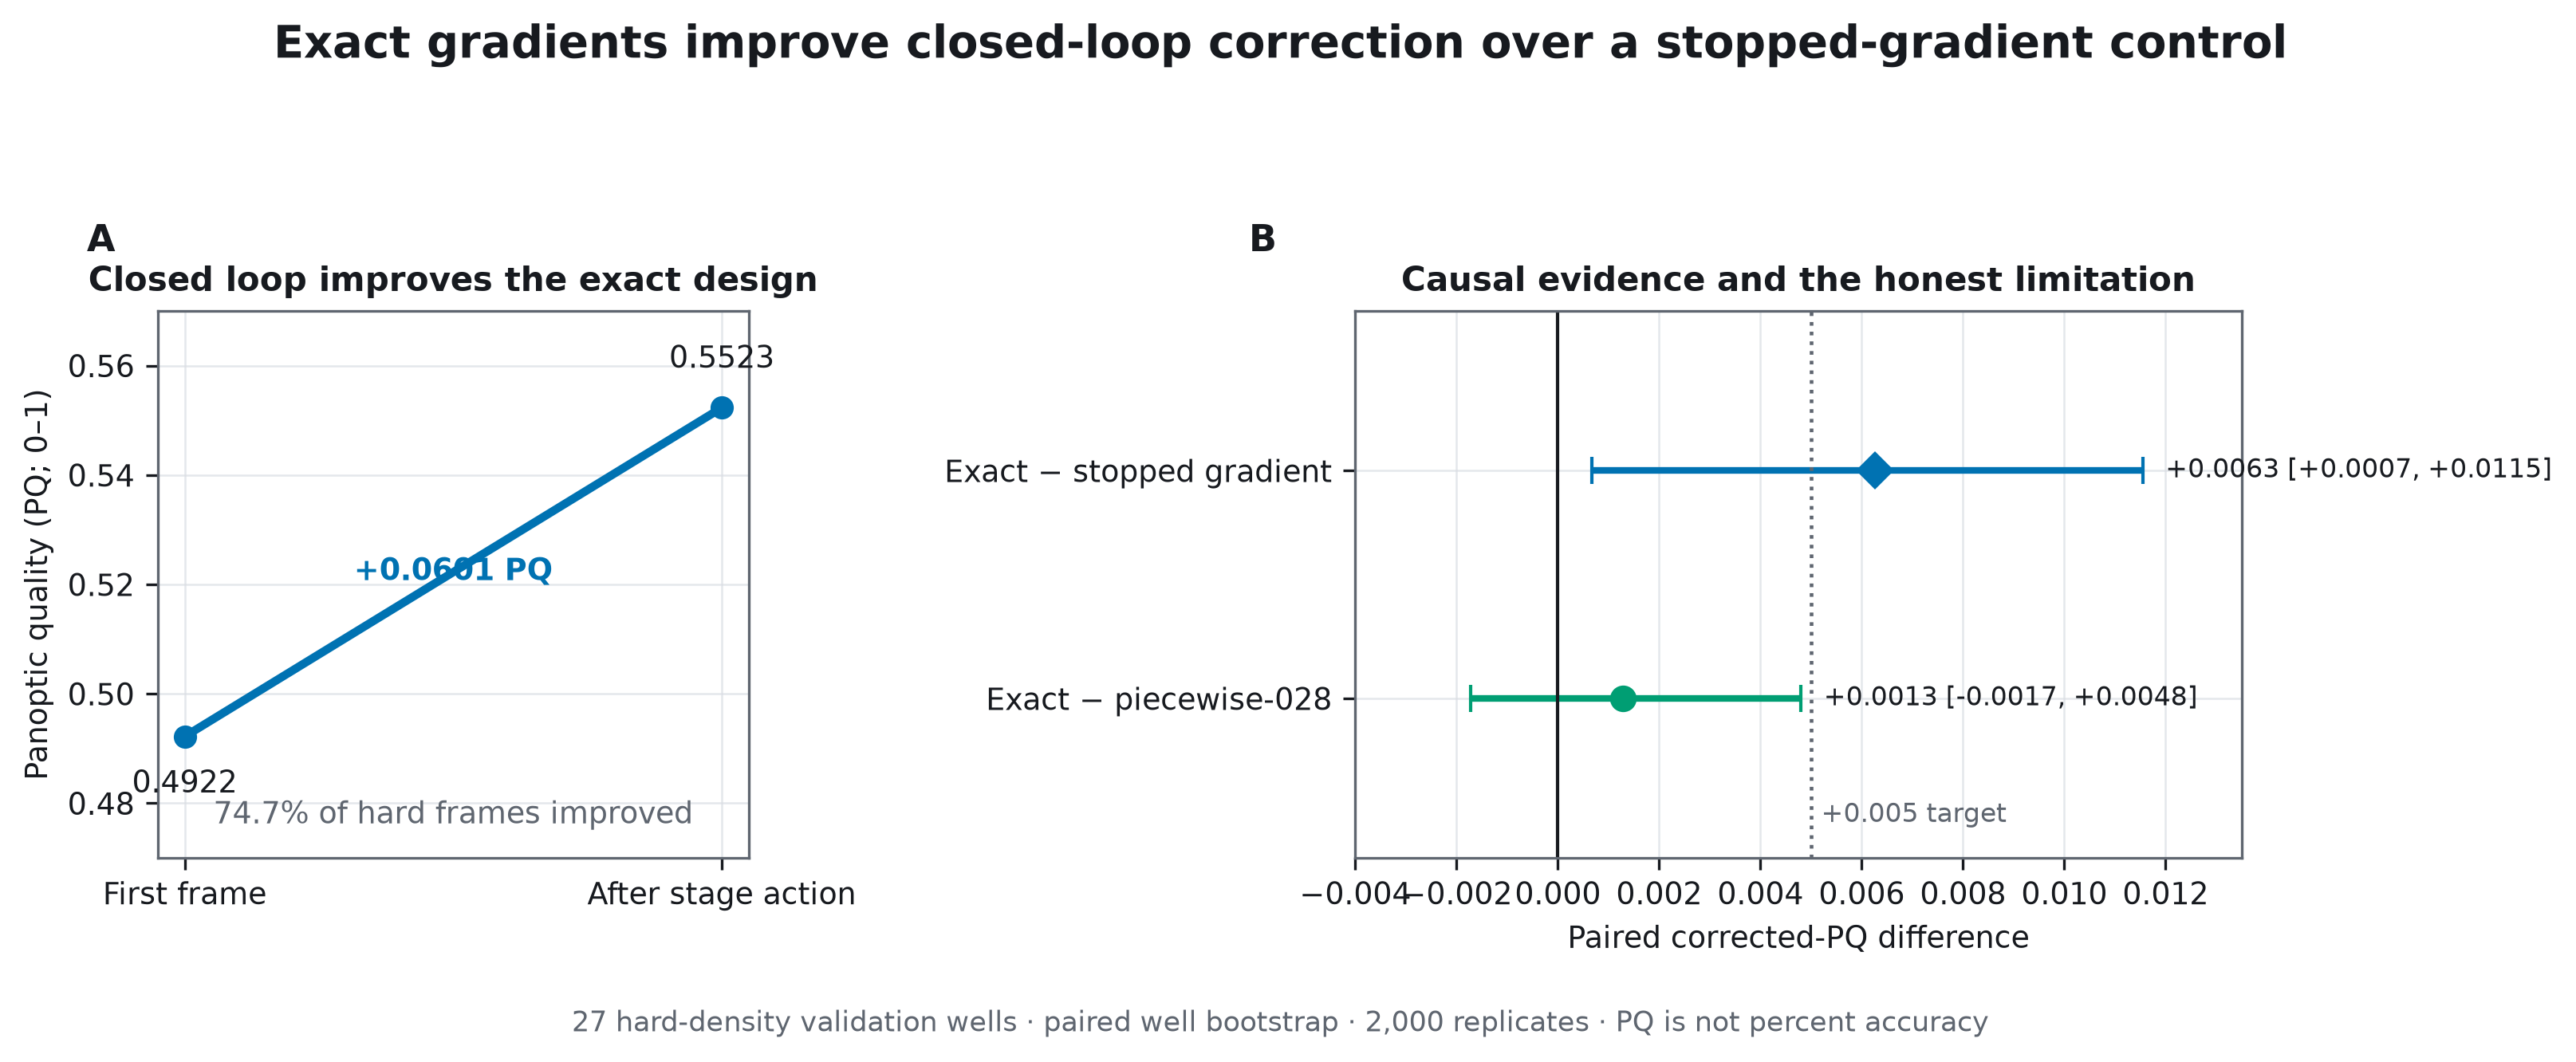
\includegraphics[width=\linewidth]{../../outputs/demo/figures/causal-comparison.png}
\end{minipage}

\textbf{What the result supports.} The balanced exact checkpoint raised corrected PQ by
0.006259 over its matched stopped-gradient pupil, with a positive paired 95\% interval.
Its own first-to-corrected PQ rose from 0.492192 to 0.552295, and 74.7\% of hard frames
improved after one predicted action.

\textbf{What it does not support.} Exact optimization beat piecewise-028 by only 0.001285
PQ; the interval crosses zero and only 55.6\% of hard wells favor exact, below the frozen
60\% stability rule. First-frame PQ also missed the segmentation-only tolerance by
0.000295. Therefore no derivative-free or locked-test branch was authorized.

\begin{tabularx}{\linewidth}{>{\bfseries}p{0.12\linewidth} X X}
\toprule
Phase & Question & Outcome \\
\midrule
v2.5 & Can exact constrained B11/B7 optimization resolve the near miss? & No endpoint passed the frozen training and soft-validation constraints. \\
v2.6 & Can controller/exposure or sequential masks create enough headroom? & Diagnostics and the complete two-mask matrix produced zero promotable candidates. \\
\bottomrule
\end{tabularx}

\scopebox{Negative follow-ups are complete experimental outcomes. They are preserved in
\texttt{docs/RESEARCH\_HISTORY.md}; they are not presented as positive results or hidden
behind the demo.}

\newpage
\section*{Reproducibility, track fit, and limitations}

\textbf{Two reproducibility levels.}

\begin{tabularx}{\linewidth}{>{\bfseries}p{0.23\linewidth} X p{0.24\linewidth}}
\toprule
Path & Command and inputs & Purpose \\
\midrule
Instant judge replay & \texttt{python3 scripts/serve\_demo.py} & Standard library only; no data, model, training, or live inference \\
Full scientific path & Python 3.12, \texttt{uv sync --frozen}, official hashed assets, three local Tesseracts & Re-run derivative, optimization, and 45-well validation into isolated checkpoints \\
\bottomrule
\end{tabularx}

The repository includes a 12.4 MiB validation replay, frozen claim matrix, JSON-pointer
traceability, SHA-256 manifests, deterministic figure builders, a committed lock file,
and output-isolation options. The full instructions are in
\texttt{docs/FULL\_REPRODUCTION.md}. The approximately 2.5 GB source subset, model
weights, virtual environment, caches, and runtime checkpoints are not committed.

\textbf{Track 05 fit.} TessScope's central artifact is differentiable image formation:
the optimized phase pupil changes a rendered fluorescence observation, which changes a
served focus decision, which changes the next rendered observation and biological task
loss. Tesseract is essential because the end-to-end derivative crosses three runtime and
framework boundaries with independently tested VJPs.

\textbf{Limitations.}
\begin{itemize}
  \item In-silico digital-twin evidence cannot establish laboratory performance,
        calibration robustness, SLM efficiency, bleaching, or motion tolerance.
  \item The supported causal effect is validation-only and is smaller than the
        preregistered improvement required over the strongest piecewise baseline.
  \item BBBC006 reference masks are automated and may contain systematic errors.
  \item The cached demo is an evidence viewer; it does not imply a production service.
\end{itemize}

\textbf{Primary sources and licenses.}
\begin{itemize}
  \item Pasteur Labs, \emph{Tesseract Hackathon 2026} and Tesseract differentiable-pipeline documentation.
  \item Ljosa et al., \emph{Nature Methods} (2012), BBBC006v1; Broad Bioimage Benchmark Collection.
  \item Deb et al., \emph{Chromatix}, bioRxiv (2025), DOI 10.1101/2025.04.29.651152.
  \item Goldsborough et al., \emph{InstanSeg}, arXiv (2024), DOI 10.48550/arXiv.2408.15954.
\end{itemize}

TessScope code and original documentation are Apache-2.0. External datasets, models,
software, fonts, and trademarks retain their own terms; see \texttt{LICENSE},
\texttt{NOTICE}, and \texttt{THIRD\_PARTY\_NOTICES.md}.

\scopebox{Submission boundary: local release candidate only. No repository push,
deployment, publication, video upload, hackathon submission, or locked-test access is
performed by this package.}

\end{document}
